\section{Bioetica 5: Le radici della professione: medicina e salute, medicina e malattia, medicina e scienza}

\subsection{Introduzione filosofica}

Mostra un'immagine delle fondamenta di Venezia, e paragona il terreno
argilloso su cui è fondata la città al terreno su cui si basa la
medicina di oggi, argilloso e alluvionale. Così come i veneziani hanno
costruito dei pali per risolvere il problema, il medico nel corso dei
secoli si è ingegnato fino ai giorni nostri dove la Medicina è basata
sulla genomica e le cosiddette scienze ``omiche''.

Il terreno argilloso su cui si basa la medicina è la filantropia, intesa
da Ippocrate come amore per il paziente e il rispetto per la sua
volontà.

Secondo Cartesio la medicina non è altro che uno dei rami della
metafisica, fisica e meccanica. La morale rappresenta la conoscenza di
tutta la realtà.

La rottura tra la medicina e la filosofia è stata traumatica, avvenuta
nell'800 quando il pensiero positivista ha reso autonoma la medicina.
Eppure fino al 1875 gli studenti di medicina erano obbligati a seguire
dei corsi di filosofia.

Ancora oggi abbiamo bisogno dei domini della filosofia, questo ce lo
dice la scienza stessa con le scienze ``omiche''.

\subsection{Perché la necessità di filosofia?}

\begin{itemize}
\item
  Per evitare di non cogliere tutte le possibilità normative del
  pensiero, con la conseguente unica disponibilità di valori per il
  medico (il paradosso del sapere scientifico ben evidente nella attuale
  crisi della medicina.

\item
  Per recuperare gli strumenti relativi ai suoi domini:

\begin{itemize}
\item[1.]
  Ontologia:lo studio dell'essere in quanto tale
\item[2.]
  Epistemologia: con cui non facciamo conoscenza scientifica
\item[3.]
  Estetica: ricerca con la sensibilità
\end{itemize}

\item
  Per rispondere alle domande se la medicina sia arte o tecnica, se si
  procede per scoperte secondo la logica scientifica o seguendo un
  processo convenzionale, naturalistico, se nella interrogazione del
  dato sia opportuno rimanere nell'ambito del riduzionismo o se non
  convenga aprirsi a visioni d'insieme, comunemente definite, anche se
  in modo generico, visioni olistiche dell'essere umano.
  \end{itemize}
  
  La filosofia è necessaria come modalità di approccio alla medicina per
  rispondere a delle domande che non tutti si pongono:

\begin{itemize}
\item
  Ritenete che sia salutare andare a lavoro in bicicletta. Che cosa
  intendete per salutare?
\item
  Dite che l'ulcera duodenale è psicosomatica. Credete quindi che il
  corpo e la mente siano due entità separate e che quella cosa che
  chiamate mente possa influenzare cambiamenti nel corpo?
\item
  Affermate che una certa terapia non è scientifica. Quali sono i vostri
  criteri per accettare una cura come scientifica?
\item
  Non ritenete che l'alcolismo sia una malattia. Che cosa intendete per
  malattia?
\end{itemize}
  
  Il medico che si pone queste domande diventa impopolare rispetto al
  medico specialista, ma dovrete avere questo modo di pensare per saper
  essere medici.

  Serve anche per evitare il rapporto conflittuale con il paziente e
  quindi gli errori nella identificazione del problema (percezione e
  intuizione), errori nella strutturazione del problema (intuizione e
  ragionamento), errori nella generazione delle ipotesi (intuizione e
  ragionamento), errore nella revisione delle ipotesi ragionamento) e
  errori nella decisione (intuizione e ragionamento).
  

  Esempio: cosa vedete in questa immagine?

   \begin{figure}[!ht]
\centering
	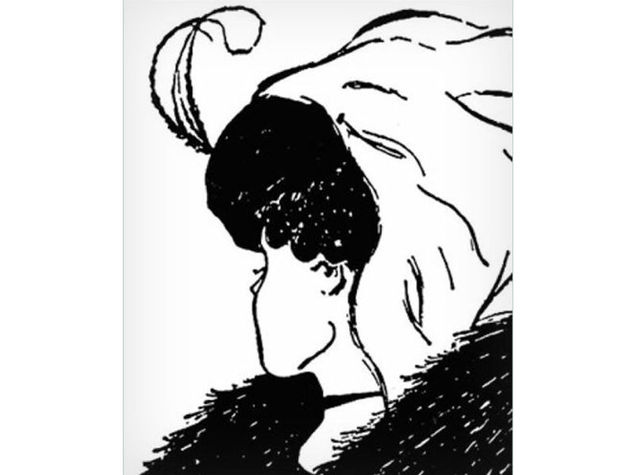
\includegraphics[width=0.8\textwidth]{33/image1.jpeg}
	\end{figure}
  
  Molti
  di voi vedono una donna ben vestita e impellicciata, ma altri vedono
  in realtà una signora anziana. Questo è un tipico esempio di errore
  medico legato all'intuizione. È facile vedere le ``facies''
  semeiologiche (ippocratica, ipotiroidea\ldots{}), ma la percezione ci
  può far fare degli errori.\\
  Le carenze della attuale formazione medica

  Nella formazione accademica si impiegano concetti quali: fatto,
  oggettività, ipotesi, teoria, legge, prova, falsificazione,
  controprova, verifica, conferma, osservazione, probabilità,
  spiegazione, esperimento, determinismo, finalismo, riduzionismo.

  Non vengono però forniti allo studente informazioni critiche sul loro
  valore e sulla reale portata di ciascuno, per cui gli si negano gli
  strumenti metodologici per sottoporre ad analisi gli scopi e i valori
  della disciplina medica.

  Si apprende in modo acritico e approssimativo concetti che
  costituiscono l'ossatura del suo modo di pensare, di un metodo di
  ragionamento che lo dovrebbe condurre sempre a privilegiare il
  confronto abbandonando assolutismi del sapere che spesso appaiono un
  ostacolo più che una risposta terapeutica.

  Questa è la filosofia! Perché la pratica medica si risolve in una
  delicata operazione conoscitiva, la diagnosi, collegata a una
  strategia che è la terapia.

  Nosologia e classificazione della malattia vanno di pari passo alla
  difficoltà di analizzare sistematicamente il procedimento diagnostico.

  \subsection{Medicina e malattia}

  Analizziamo il concetto di malattia: nonostante questo sia centrale in
  medicina, non esiste una definizione accettata dalla comunità dei
  medici e degli operatori sanitari.

  Anche se non chiarito, il concetto inoltre regola in qualche modo la
  soglia di intervento della medicina e dei sistemi sanitari.

  Quindi in realtà è una famiglia di significati concettualmente
  imparentati riferentesi a un insieme di fenomeni accostati sulla base
  di vari interessi di tipo pratico e sociale.

  Non è una conseguenza del riconoscimento di una comune struttura
  concettuale o del fatto che il concetto ha il suo riferimento in uno
  specifico oggetto o processo della natura.

  Quindi come definiamo questo concetto? Sarebbe auspicabile per
  migliorare la metodologia di indagine sulle condizioni morbose e le
  logiche della spiegazione della malattia, con conseguenti benefici
  anche sui versante pratico della prevenzione e del trattamento di
  condizioni patologiche.

  Il concetto è complesso perché la malattia è associata a una
  esorbitante varietà di attributi, peraltro riferiti a dimensioni di
  fenomeni molto lontani tra di loro. Per esempio la malattia è:

\begin{itemize}
\item
  Disfunzione fisica, dolore non causato da ferite o traumi,
  debilitazione progressiva;
\item
  Processo o struttura statisticamente abnorme;
\item
  Condizione per cui esiste o viene scoperta una cura, per cui è
  possibile la rilevazione per mezzo di una tecnologia diagnostica (può
  essere rilevata prima dei sintomi)
\item
  Una deviazione dal normale funzionamento sociale e lavorativo;
\item
  Una condizione per cui viene scoperto un agente eziologico\ldots{}
\end{itemize}

  \subsubsection{Le malattie costituiscono generi naturali?}

  Se la malattia costituisse un genere naturale le malattie dovrebbero
  condividere una qualche particolare natura o proprietà, ma ciò non si
  verifica. Si sa a priori che anche se tutte le malattie condividessero
  una particolare natura, questo non dimostrerebbe ancora che una
  malattia consiste nell'avere una particolare natura.

  Esempio di Koch, che affermava che ad ogni malattia corrisponde un
  patogeno, ma questo sappiamo non essere vero. L' idea che il concetto
  di malattia abbia un riferimento ad una condizione con una particolare
  natura, è diffusa nell'opinione pubblica comune, ma non rara anche tra
  i medici e in certe posizioni dell'epistemologia della medicina, come
  quelle emerse con l'avvento della microbiologia ovvero quelle
  biostatistiche proposte più recentemente. La storia della medicina
  dimostra che le condizioni di interesse medico possono passare da una
  categoria all'altra col modificarsi delle conoscenze e delle teorie.

  Come facciamo a distinguere il fisiologico dal patologico? Il filosofo
  francese Canguilhem scrive: ``Il concetto di norma è un concetto
  originale che non si lascia, in fisiologia, ridurre a un concetto
  oggettivamente determinabile con metodi scientifici. Non si dà una
  scienza biologica del normale, ma si dà una scienza delle situazioni e
  delle condizioni biologiche normali. Ogni concetto empirico di
  malattia si rapporta al concetto assiologico della malattia. Non è, di
  conseguenza, un metodo oggettivo che fa qualificare come patologico un
  fenomeno biologico considerato. È sempre la relazione dell'individuo
  malato, tramite la medicina della clinica, ciò che giustifica la
  qualificazione di un fenomeno come patologico.

  Anche ammettendo l'importanza dei metodi oggettivi di osservazione e
  di analisi in patologia, non sembra che si possa parlare,
  correttamente dal punto di vista logico di una patologia oggettiva.''

  Altro esempio è la colonizzazione del tratto gastro intestinale dei
  bambini da parte dei lattobacilli, il quale è un processo normale che
  protegge dall'azione patogena di E.Coli . Cosa distingue
  biologicamente questa colonizzazione batterica da altre come quelle
  del tetano, che invece portano alla malattia?

  Siamo di fronte alla contraddittoria situazione che uno stesso
  processo biologico, l'infezione, causato da una stessa classe di
  microrganismi, può essere un fattore fondamentale della norma
  biologica, della salute, o un elemento eziologico per una malattia
  mortale.

  Quindi il concetto di relatività del patologico: una certa condizione
  sia patologica che fisiologica dipende non soltanto dalla sua natura
  ma anche dalle interazioni che un organismo intrattiene con le altre
  specie e con l'ambiente in cui vive. La talassemia conferisce maggiore
  resistenza alle infezioni malariche e costituisce quindi un vantaggio
  in un ambiente dove la malaria è endemica. Le malattie genetiche sono
  espressione di processi storici, per percorsi evolutivi singolari e
  irripetibili, frutto di una selezione che agisce sulla base di
  dinamiche ambientali e etologiche sempre cangianti o a partire da
  mutazioni casuali.

  Per questa ragione è sempre possibile immaginare un contesto
  ambientale, un sistema di rapporti intra- e interspecifico dove una
  determinata mutazione patologica non porta alla malattia o risulta
  addirittura vantaggiosa.

  Un'altra ragione a sostegno dell'idea che le condizioni patologiche
  non costituiscono un genere naturale distinto dalle condizioni
  normali, è che certe malattie sembrano staccarsi dalla normalità
  soltanto per differenze di grado relative a certe variabili.

  Un esempio è l'ipertensione (prima definita essenziale, cioè parte
  della vita). Pur ancora largamente incompresa nella sua
  eziopatogenesi, l'ipertensione è certamente considerata una condizione
  patologica.

  Tuttavia essa si distingue dalla normalità soltanto in ragione di una
  deviazione quantitativa e qualitativa.

  Tutto ciò ha portato Grmek a definire il concetto di Patocenosi,
  accorpando un complesso di malattie variabili quali e
  quantitativamente in cui la frequenza di ognuna dipende dalla
  frequenza delle altre e da fattori ambientali.

  {[}Dalla slide --\textgreater{} Patocenosi = insieme delle malattie
  presenti in una popolazione in un determinato ambiente e in una data
  epoca (Gmek), in altre parole: insieme dei dati epidemiologici stabili
  in una popolazione e paradossalmente corrispondente allo stato di
  salute di una popolazione{]}

  La medicina è in gran parte una costruzione ideologica, il medico che
  crede di interpretare la malattia in modo oggettivo in realtà si
  confronta con tre istanze storicamente preponderanti:

\begin{itemize}
\item
  Medica di oggettività scientifica, che fa riferimento
  all'epistemologia positivista o alla tradizione empirista che situano
  al centro dell'indagine le malattie e i processi fisiologici.
\item
  Pubblica di salvaguardia e promozione del benessere dei cittadini
\item
  Privata intimamente legata all'empowerment del paziente.
\end{itemize}

  Questo concetto è presente anche nella medicina scientifica, noi
  crediamo che sia giusta al 100\% ma anche nella medicina scientifica ,
  la malattia resta una nozione legata a fattori storici, culturali ed
  etici; basti pensare al confine tra normale e patologico che varia nel
  tempo e in funzione dei modelli di spiegazione e delle tecniche di
  rilevazione dei segni e dei sintomi.

  La medicina ha esteso il suo dominio in che modo?

\begin{itemize}
\item
  Sul piano quantitativo: abbassamento della soglia (es. colesterolo)
\item
  Sul piano temporale : diagnosi precoce
\item
  Sul piano qualitativo: nuove malattie
\end{itemize}

  Questo concetto è interesse di molti, come il Disease Medical Journal
  che lo descrive con la frase: ``si possono fare molti soldi dicendo
  alle persone sane che sono malate''.

  \subsubsection{Conclusioni}

  Nonostante il concetto di malattia sia centrale in medicina, non
  esiste una definizione comunemente accettata dalla comunità dei medici
  e dagli operatori sanitari.

  Le condizioni patologiche non sono dei generi naturali e per questo
  non possono distinguersi con precisione e certezza dalle condizioni
  normali.

  Dalla seconda metà dell' ottocento le medicina ha assimilato il
  paradigma scientifico riduzionistico e meccanicistico delle scienze
  fisico-chimiche.

  Ma anche nella medicina scientifica la malattia resta una nozione
  legata a fattori storici e culturali ed etici perché il confine tra
  normale e patologico varia nel tempo e in funzione dei modelli di
  spiegazione e delle tecniche di rilevazione dei segni e dei sintomi.

  Ma anche se non chiarito, questo concetto regola in qualche modo la
  soglia di intervento della medicina e dei sistemi sanitari e dimostra
  come queste considerazioni filosofiche che permeano tuttora il
  pensiero medico, poco impattano l'attività del medico proprio per la
  natura pratica ed empirica della medicina.

  \subsection{Medicina e salute}

  Parliamo del concetto di salute, se io interrogassi ognuno di voi, non
  molti riuscirebbero a dare un significato. In genere viene definito
  per negazione (salute come assenza di malattia), per molte persone
  star bene vuol dire non essere malato. Questo significa però eliminare
  la persona da questo processo, cioè il fatto che la malattia si
  subisca senza fare niente e significa non ammettere l'esistenza di
  segni di processi patologici.
\\\\
  Come superare questa posizione riduzionista?

  La posizione dell'OMS è che ``la salute è uno stato di completo
  benessere fisico, mentale e sociale, e non consiste soltanto in
  un'assenza di malattia o di infermità.'' Questa definizione è stata
  inserita nella Costituzione Italiana e costituisce l'articolo 32 : ``
  La Repubblica tutela la salute come fondamentale diritto
  dell'individuo e della collettività e garantisce cure garantite agli
  indigenti''

  L' igienista Seppilli afferma `` La salute è una condizione di
  armonico equilibrio funzionale, fisico e psichico dell'individuo,
  dinamicamente integrato nel suo ambiente naturale e sociale.''

  L'OMS ha rivisto e migliorato il concetto di salute negli anni (1977)
  affermando che `` nei decenni futuri l'obiettivo sociale principale
  dovrebbe essere di far raggiungere a tutta la popolazione entro il
  2000 uno stato di salute che permetta di vivere una vita socialmente
  ed economicamente produttiva''.

  Lo stesso ha affermato la Carta di Ottawa il 21 novembre del 1986 ``la
  buona salute è la principale risorsa per lo sviluppo sociale,
  economico e personale ed è un' importante dimensione di qualità della
  vita. I fattori economici, politici, sociali, culturali, ambientali,
  comportamentali e biologici possono favorire la salute o danneggiarla.

  Noi medici ci abbiamo messo molti anni per introdurre questi concetti
  nel nostro codice deontologico.

  \subsubsection{Tradizionale modello medico di salute}
  
  Ogni malattia ha una causa biologica primaria, oggettivamente
  identificabile( deviazione dalla norma di variabili biologiche
  misurabili).

  Nella diagnosi non entrano fattori comportamentali e
  socio-psicologici, che vengono spiegati con processi biochimici e
  neurofisiologici disturbati e non come cause potenziali di malattia.

  Questo modello deve essere superato! Le conseguenze sono:
  
\begin{itemize}
\item
  Concede poco spazio all'azione preventiva (volta a ridurre l'incidenza
  delle malattie croniche tramite cambiamenti nelle credenze,
  atteggiamenti e comportamenti relativi alla salute)
\item
  Enfatizza il potere attivo degli operatori sanitari, promuovendo una
  posizione passiva nel paziente
\item
  Fornisce una visione riduzionistica: i fenomeni complessi derivano da
  un singolo principio primario
\item
  Implica un dualismo mente/corpo: per cui il mentale viene separato dal
  somatico
\end{itemize}

  \subsubsection{Modello biopsicosociale di salute}

  Questo modello ha avuto come massimo interprete lo psichiatra
  statunitense Engel che approfondisce il livello psicologico e sociale.
  Ci si orienta sulla salute globale della persona nel suo ambiente; si
  enfatizza la promozione della salute e la prevenzione di malattia; si
  tiene conto delle necessità di interazione o integrazione tra i vari
  livelli di analisi (interdisciplinarietà) e i diversi ruoli
  professionali (multiprofessionalità). Quindi salute come sistema
  integrato!

  Conseguenze:
\begin{itemize}
\item
  Psiche e corpo sono indivisibili
\item
  Si sottolinea il carattere dinamico del rapporto tra individuo e
  ambiente, sottolineando l'instabilità di esso. Un individuo viene
  considerato sano quando è in armonia con l'ambiente interiore ed
  esteriore, e malato quando è in disarmonia.
\item
  Messa in evidenza dell'influenza sullo stato di salute di fattori
  ambientali e sociali ( fame, disoccupazione, emarginazione\ldots{})
\item
  La salute non è solo benessere derivante dal funzionamento
  dell'organismo ma anche il risultato dell'interazione con l'ambiente.
\end{itemize}

  Il concetto di sociale consiste nelle norme sociali di comportamento
  (fumare, promiscuità sessuale\ldots{}.), pressioni a cambiare il
  proprio comportamento da parte della società, valore sociale della
  salute, classe sociale, appartenenza etnica e altre variabili come
  lavoro, coesione sociale\ldots{}

  Quindi la definizione di salute dell'OMS rende difficile, se non
  impossibile, porre dei limiti alla pratica medica, perché una volta
  incluso il concetto di benessere nella definizione, molti interventi
  medici potrebbero essere giustificati appellandosi a questo aspetto
  molto soggettivo, mai quantificabile o misurabile.

  L'obiezione più forse quindi è che nel concetto di salute è stata
  inserita proprio la salute sociale. Così la medicina è indotta ad
  occuparsi di aspetti della vita umana che prima non erano presenti
  nella sua agenda (es. la chirurgia estetica per cercare il consenso
  sociale).

  Quindi attenzione medico, a non arroccarti su posizioni arbitrarie
  quando si adotta un concetto di salute univoca e stabile. Quando si
  parla di salute dobbiamo confrontarci con un arcipelago di idee e
  significati ma anche atteggiamenti culturali che divaricano dalla
  dimensione empirica dei fatti biologici e dalle prove di efficacia su
  cui tanto ci affidiamo nella pratica della medicina moderna.

  Il rapporto tra salute-medicina e filosofia è molto forte. Oggi il
  limite della medicina è il rapporto che esiste tra l'evento patologico
  e il miglioramento della situazione creato da questo.

  \subsection{Medicina e scienza}

  Nella pratica clinica questi due campi (medicina e scienza) si
  presentano sempre più intrecciati e tendono ad assumere pertanto
  contorni sfumati ed incerti di conseguenza un' indagine sulle finalità
  e valori della prima deve tenere in considerazione gli scopi e il
  substrato culturale della seconda.

  La verità scientifica anche in medicina ovvero quello che, agli occhi
  di un medico rispetto ad un malato, è scientificamente vero, giusto,
  appropriato o adeguato dipende da:
\begin{itemize}
\item
  Come si conosce un malato!
\item
  Da chi conosce questo malato!
\item
  Dal contesto in cui si conosce!
\end{itemize}

  Tutto questo è espresso nel mondo anglosassone, da tre termini:
  \begin{itemize}
\item
  OGGETTIVO (DISEASE): la malattia del medico, cioè la
  concettualizzazione della malattia da parte dei medici, il modello che
  il medico ha della malattia.
\item
  SOGGETTIVO (ILLNESS): la malattia del malato, il sentirsi malato, che
  include aspetti di esperienza soggettiva dello star male,
  culturalmente mediata.
\item
  RELAZIONE (SICKNESS): il riconoscimento sociale della malattia, cioè
  la rappresentazione che ha la società della malattia.
\end{itemize}

  Quindi il sapere e conoscere in medicina ha alla base due aspetti: uno
  scientifico e l'altro clinico. I greci chiamavano la medicina iatrikè
  tekne, in contrapposizione ad episteme, una specie di attività
  artigianale che opera la sintesi tra scienza, tecnica e arte.
  \begin{itemize}
\item
  Scienza, come conoscenza organizzata di tutte le circostanze relative
  alla salute dell'uomo.
\item
  Arte in quanto capacità di applicare tale conoscenza alla cura della
  malattia.
  \end{itemize}

  Si può pertanto distinguere nella scienza in Medicina tra ciò che deve
  essere fatto (conoscenza pratica) ed il perché deve essere fatto
  (conoscenza teorica).

  Vediamo un po' di aforismi a riguardo:
  \begin{itemize}
\item
  La medicina.....''un'area della sfera applicativa umana in cui
  scienza, pensiero esistenziale e etica felicemente si incontrano.''
\\\\
  Mario Austoni
\item
  La medicina è ``una scienza sociale e la politica non è altro che la
  medicina pensata in grande.''
\\\\
  Rudolf Virchow
\item
  ``La Medicina per la sua natura biologica è realmente una robusta arte
  di una debole scienza.''
\\\\
  Milos Jenicek
\end{itemize}

  \subsubsection{Il medico coltiva una scienza e pratica un'arte}

  Imporatnti corollari:
  
\begin{itemize}
\item
  La medicina esiste per curare le persone perchè si sentono malate, e
  non soltanto perchè sono riconosciute tali.
\item
  La medicina non una scienza come tutte le altre, in quanto include
  regole e leggi naturali e soggettività, dimensioni biologiche e
  psicologiche.
\end{itemize}

  Definire lo status attuale della Medicina è indubbiamente difficile.
  Infatti è in uno stato 'transizionale', ai mondi della società e della
  scienza contemporaneamente.

  Si trova anche in uno stato 'non chiaro', per il combinarsi di forze
  eterogenee multidisciplinari e multidimensionali, che rendono la
  realtà attuale della medicina di difficile definizione e che possono
  progredire verso un' evoluzione la cui portata non è del tutto
  precisabile.

  \subsubsection{La medicina nella storia}

  Quindi dobbiamo capire che la medicina poggia su un terreno argilloso
  alluvionale ma nel corso dei secoli sono stati piantati dei paletti, i
  quali devono diventare per noi una forma mentis.

  La medicina si rapporta alla società e alla storia attraverso degli
  ``scenari magistrali'', ovvero cornici concettuali nel corso della
  storia della Medicina.

  Ora vorrei farvi una breve carrellata sulla storia giusto per farvi
  capire come siamo arrivati alla medicina post-genomica che
  caratterizza i nostri giorni e il futuro della Medicina.

  Inizialmente la medicina era quella ``omerica'' cioè la malattia era
  considerata una punizione divina e quindi una debolezza ( gli eroi
  omerici non potevano essere malati).

  La vera storia della medicina però comincia con Ippocrate e la sua
  medicina razionale.

  La nascita della medicina razionale in Grecia nell'epoca classica, al
  momento stesso della nascita dell'arte e della filosofia, pone come
  elemento epistemologico discriminante la riflessione sulla causalità e
  sull'ordine delle cose. Secondo Ippocrate l'uomo era il finalismo
  della natura! Lui, ma anche Galeno, applicano la Dottrina Umoralista
  che dice:

  ``La salute è garantita dall'equilibrio tra umori interni (microcosmo)
  e l'ambiente naturale circostante (macrocosmo)''

  \begin{figure}[!ht]
\centering
	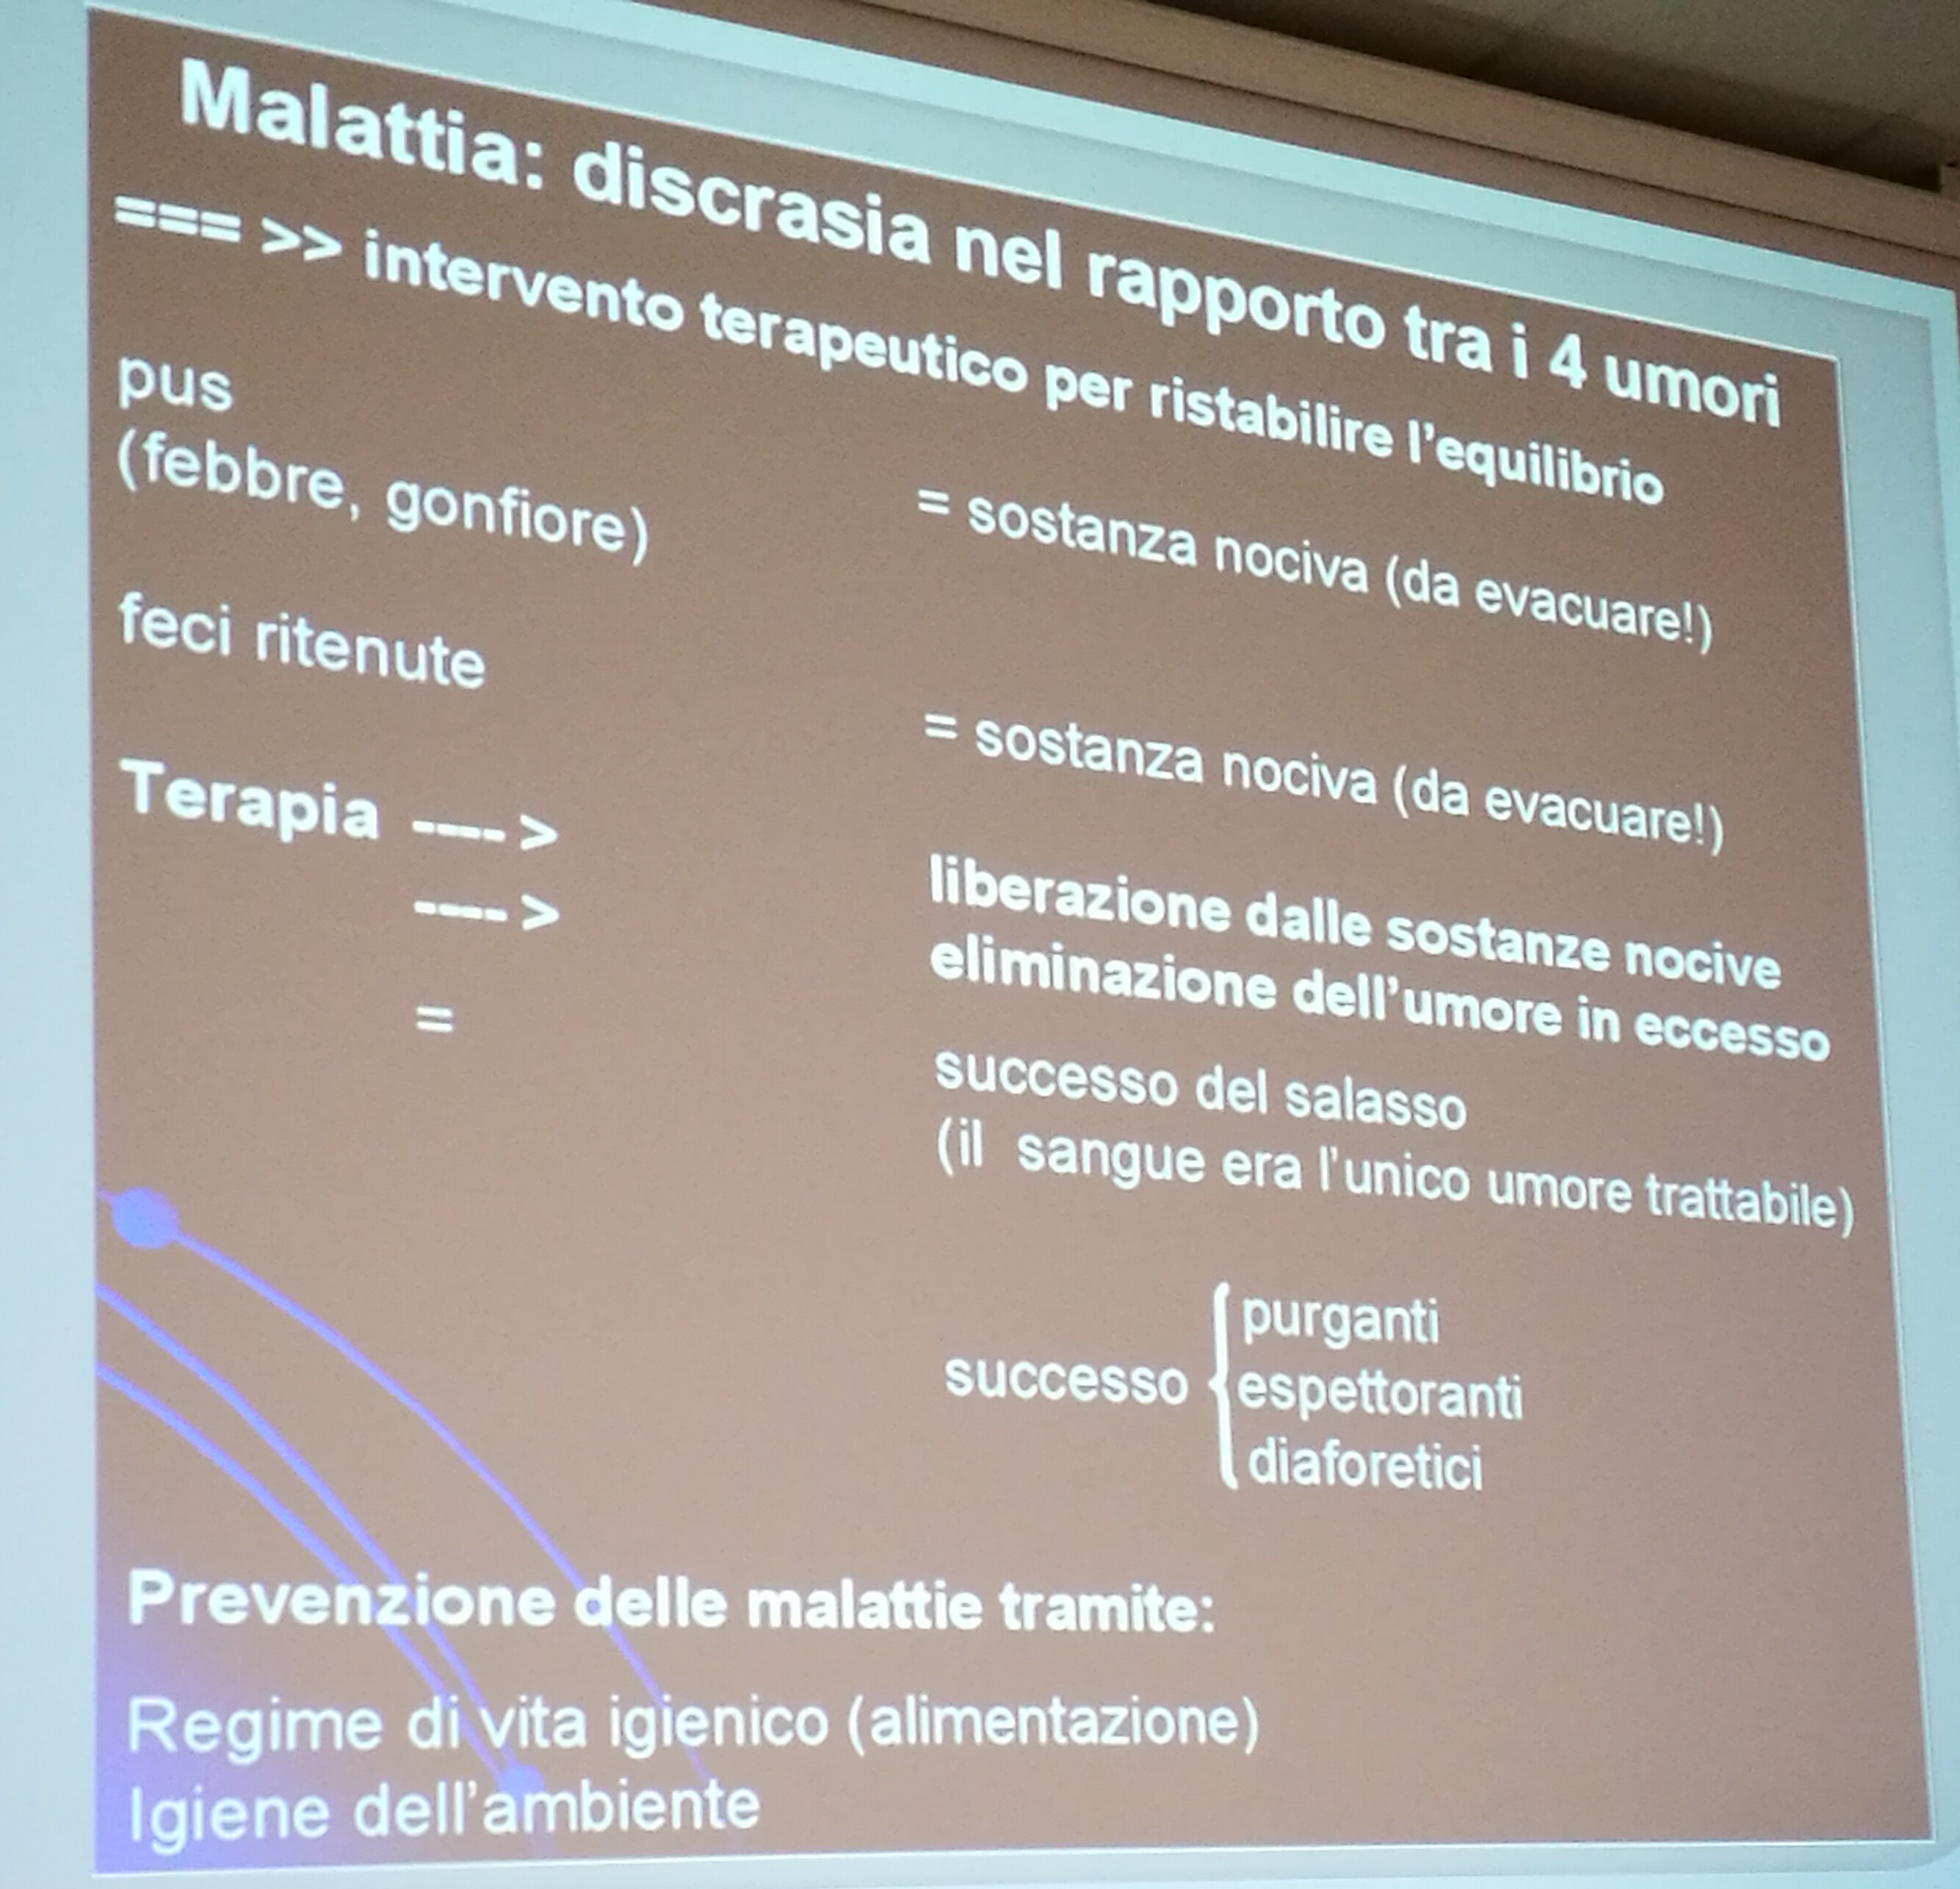
\includegraphics[width=0.8\textwidth]{33/image2.jpeg}
	\end{figure}

  Quindi la funzione del medico è di riordinare questi umori, ad esempio
  togliere il pus o fare i salassi (pratica messa in atto fino metà del
  '900).

  Galeno sviluppa un po' di più questo concetto ma comunque rimane
  fedele all'ambito micro- e macrocosmo. Aggiunge osservazioni ottenute
  da esperienze anatomo-comparative, quindi c'è una primordiale idea di
  sperimentare. L'architrave del suo pensiero è il concetto aristotelico
  in cui Dio opera dall'esterno del mondo quale Motore Immobile.

  La medicina classica quindi si basa su fondamenti della logica che
  sono gli strumenti per gli insegnamenti che non devono essere mai
  messi in dubbio.

  La causa della malattia resta legata all'empirismo e all'esperienza
  del singolo. Il medico è timoniere e allontana il paziente dagli
  scogli e dalle tempeste ma lasciando agire la natura.

  \paragraph{Cenni sull'articolazione epistemologica fino all'epoca moderna}

  Si possono suddividere tre livelli o piani di conoscenza:
  
\begin{itemize}
\item[1.]
  un piano osservativo e sperimentale qualitativo
\item[2.]
  un piano razionale e speculativo
\item[3.]
  un piano gnostico basato sulla verità rivelata
\end{itemize}

  Un pensiero rivoluzionistico lo ebbe Guglielmo di Ochkam, un teologo
  francescano, che ha cambiato il pensiero medioevale. Secondo Ochkam
  non c'è nessun rapporto tra i contenuti di fede e quanto la ragione
  dimostra essere vero, anzi gli articoli della fede appaiono a volte
  falsi e irrazionali agli occhi della sola ragione. Dunque la teologia
  non era più considerata come una scienza ma solo un insieme di verità
  necessarie all'uomo per conseguire la vita eterna.

  Si assiste al superamento dello ``scenario magistrale'' della medicina
  classica

  Si subordina il caso individuale alla conoscenza di spiegazioni
  universali.

  La pratica medica deve basarsi sulla conoscenza scientifica delle
  leggi generali del normale e del patologico. Quindi inizia a
  delinearsi la medicina scientifica e basata sulle evidenze.

  Il primo a criticare il pensiero di Galeno fu Vasalio, il quale trovò
  200 errori nell'anatomia di Galeno, autorità indiscussa per secoli.

  Dal rinascimento in poi la visione divenne antropologica, cioè il
  paziente è messo al primo posto.

  La malattia, tramite la morfologia, la patologia,e la ricerca
  etiologica, da un punto di vista ontologico, acquisisce una precisa
  concretezza e si impone come quadro attualmente accettato.

  Nel `700 con Morgagni nasce l'anatomia patologica: mette in relazione
  le alterazioni anatomiche con quelle patologiche e dimostra che per
  ogni alterazione anatomica c'è un'alterazione della funzione.

  Marie Bichat: riprende la lezione del Morgagni e scopre che gli organi
  del corpo umano sono costituiti da tessuti.

  Vircow: sviluppa i moderni concetti della patologia cellulare e della
  patogenesi delle malattie e sviluppa il concetto che le malattie
  nascono dalle cellule in primis.

  Con queste nuove basi si arriva al metodo scientifico che si avvale di
  3 fasi:
\begin{itemize}

\item[1.]  Fase induttiva

\item[2.]  Fase deduttiva

\item[3.]  Fase di controllo o sperimentale

\end{itemize}

  Per Popper un'ipotesi o una tesi è teoria scientifica solo se può
  essere sottoposta a ``falsificazione'' o è falsificabile.

  \paragraph{L'era post genomica e le scienze ``omiche''}

  Una delle scoperte più eclatanti della nuova era post-genomica, è che
  il paradigma secondo cui un gene codifica una sola proteina risulta
  non essere più valido.

  A causa di modifiche post-traduzionali (glicosilazione,
  fosforilazione) delle proteine, a un genoma possono corrispondere più
  di un proteoma.

  Il genoma di un essere vivente, anche quando completamente
  sequenziato, non permette di comprendere tutte le funzioni biologiche
  che caratterizzano un organismo e che dipendono da molteplici fattori,
  tra i quali le vie regolatorie metaboliche delle proteine.

  Questo che conseguenze ha? Ognuno di noi è un'entità irripetibile e da
  ciò scaturisce la necessità di una medicina personalizzata.

  Di questo si occupano le scienze post-genomiche dette anche ``omiche''
  (trascrittomica, proteomica, metabolomica), le quali hanno
  rivoluzionato e rivoluzionano l'approccio della biologia allo studio
  delle malattie. Il compito di queste nuove discipline è quello di
  decifrare la complessità dell'informazione genetica utilizzando
  tecnologie di ultima generazione.

  Una persona non può essere definita unicamente in base alla sequenza
  genomica ereditata al momento del concepimento (la vecchia idea del
  determinismo genetico)

  La medicina post-genomica sta superando il tradizionale approccio
  ``riduzionistico'' muovendo verso una visione olistica, quella della
  ``medicina dei sistemi'', che, in maniera interdisciplinare, guarda al
  corpo umano come ad un insieme integrato, il quale incorpora le
  complesse interazioni genomiche,ambientali e comportamentali.

  \paragraph{La medicina personalizzata}

  ``I dieci farmaci con il maggiore fatturato negli Stati Uniti
  funzionano , nel migliore dei casi , in un paziente su quattro''( nel
  peggiore in uno su 25 dalla rivista di Nature). Perchè? Perchè ognuno
  di noi metabolizza in un modo diverso e questo è alla base della
  ``Precision Medicine''.

  La `` personalizzazione'' della medicina o in termini anglosassoni
  ``Precision Medicine'' ci ripropone vecchi problemi che sembravano
  risolti con la proposta dei cosiddetti studi randomizzati per valutare
  l'efficacia dei trattamenti.

  \begin{figure}[!ht]
\centering
	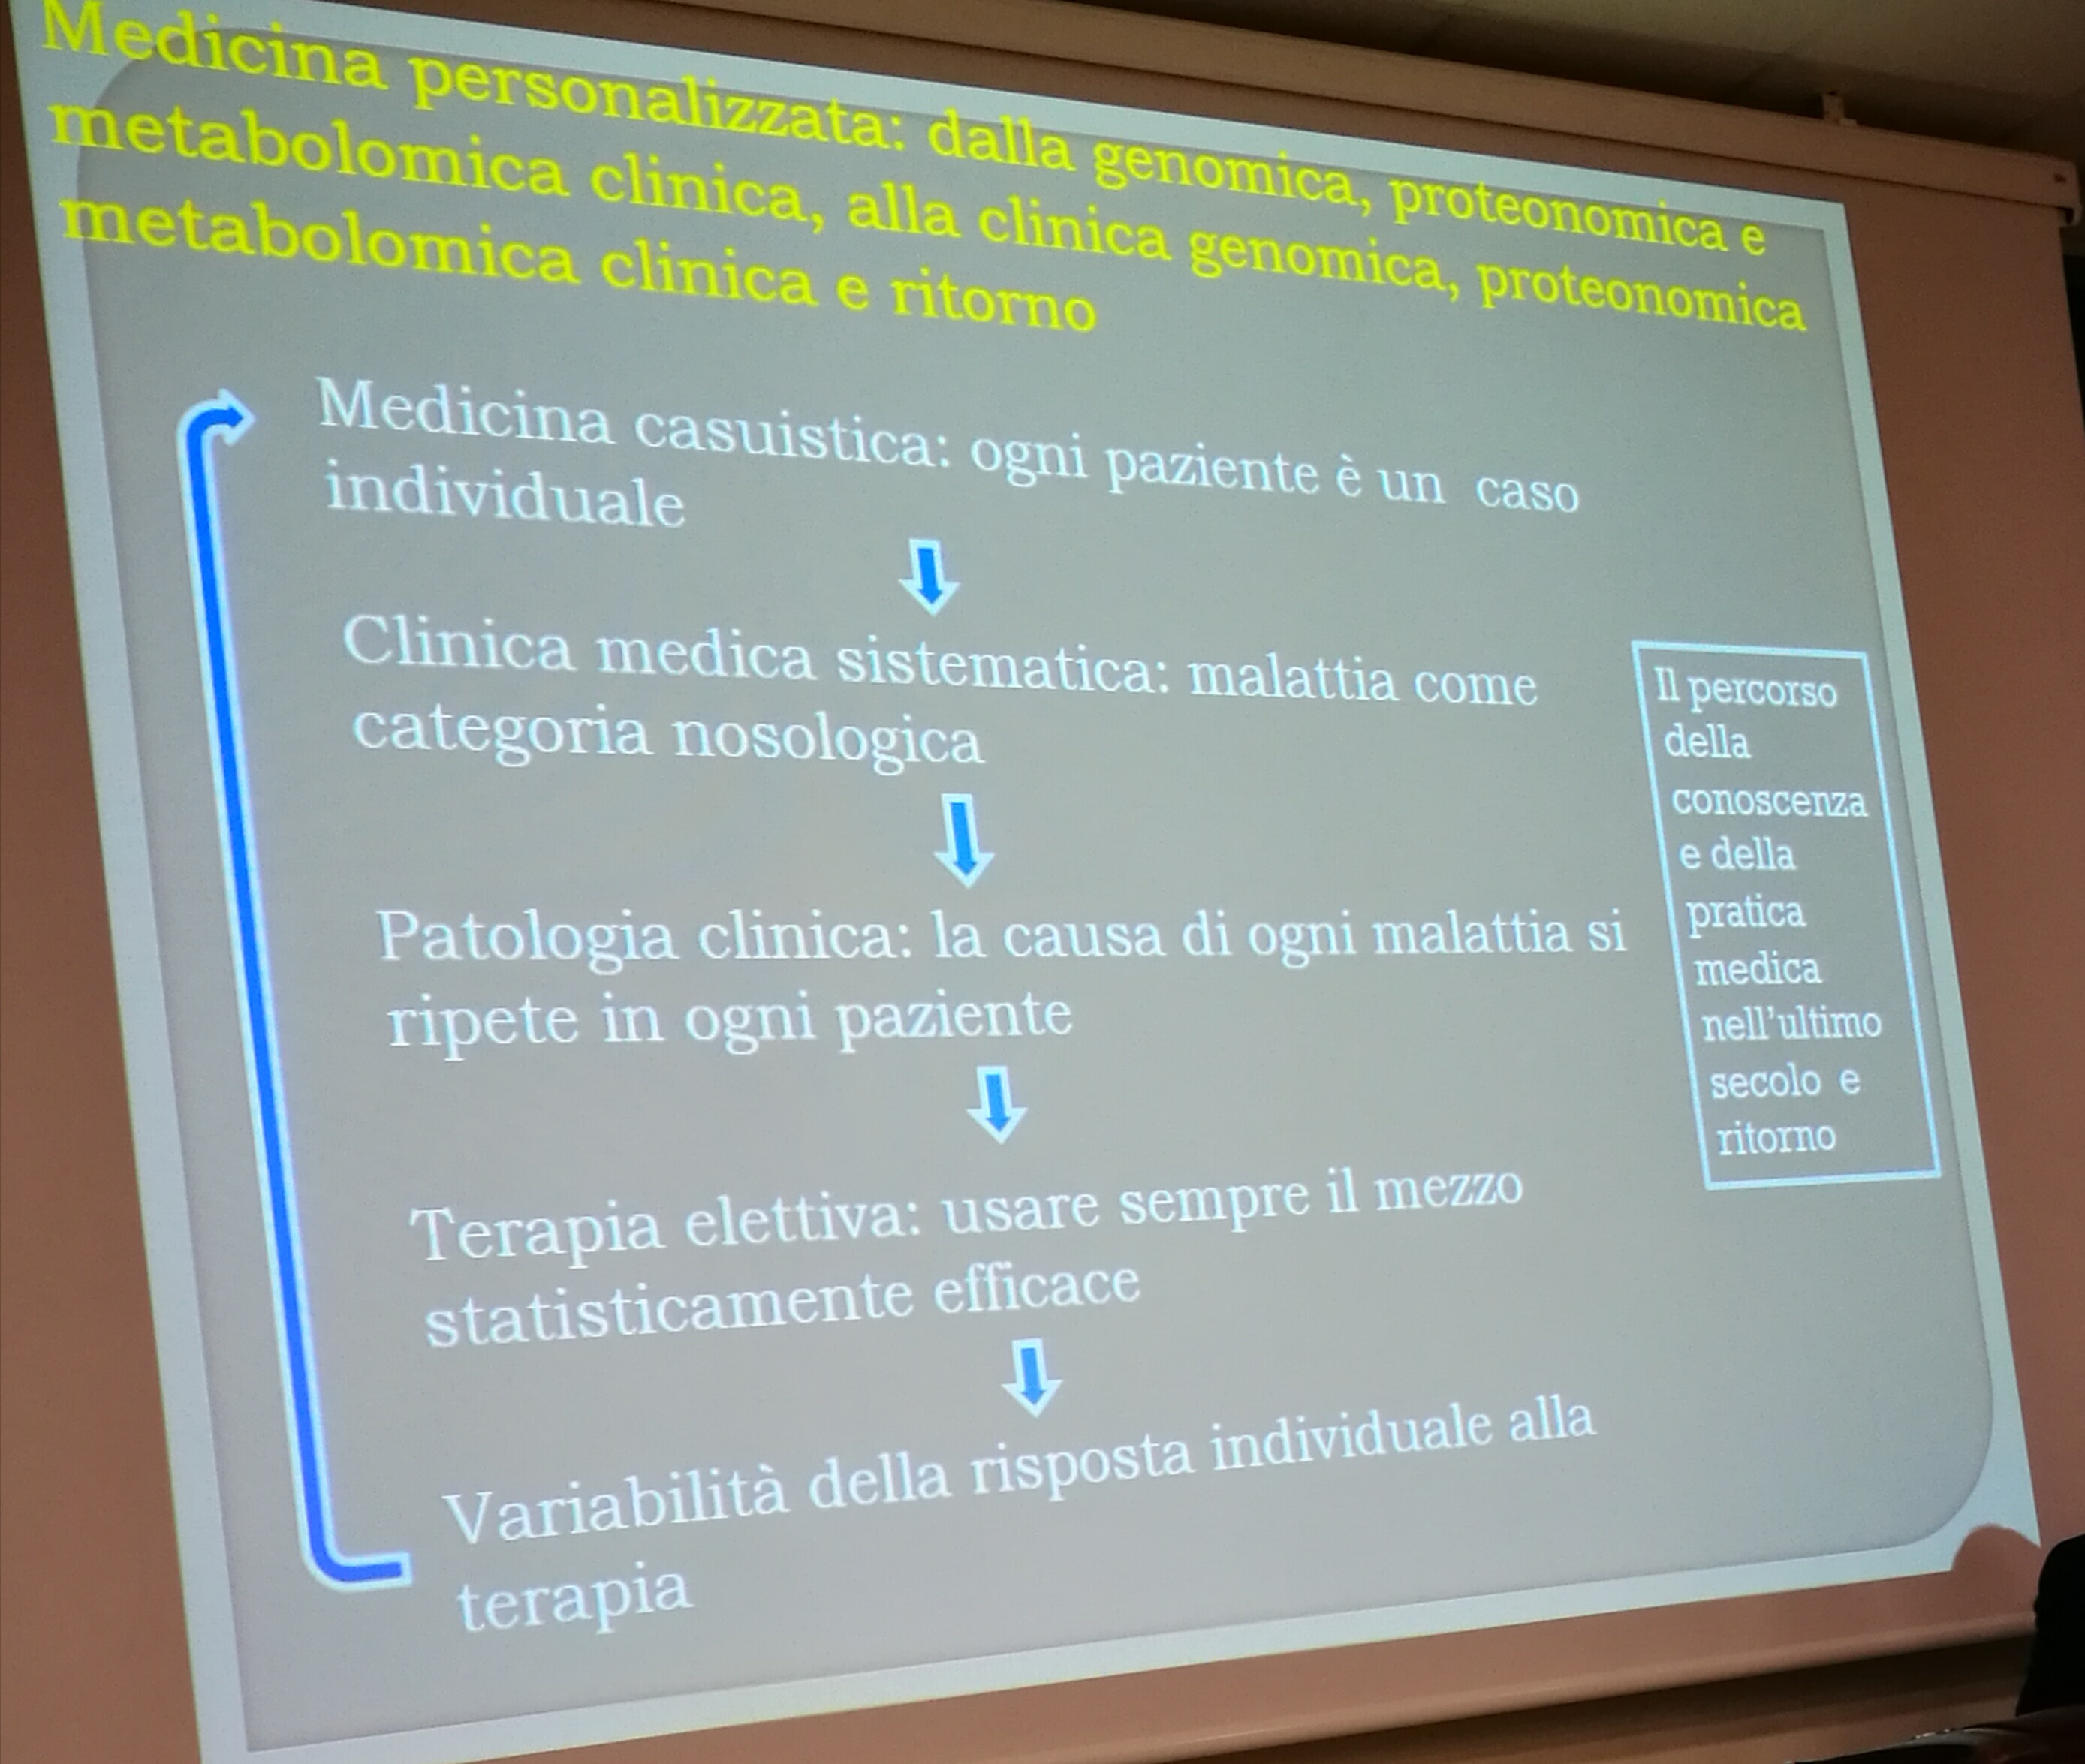
\includegraphics[width=0.8\textwidth]{33/image4.jpeg}
	\end{figure}

  \subsubsection{Filosofia e metodo scientifico...un nuovo cambio di prospettiva}

  Torniamo al discorso iniziale e lo arricchiamo con tutto quello detto
  fin ora.

  Dobbiamo constatare che le problematiche filosofiche , logiche e
  ontologiche oggi emergono nelle scienze non come una giustapposizione
  esterna, facoltativa , estranea al metodo scientifico stesso ma
  dall'interno delle stesse quale problema scientifico
\begin{itemize}
\item per un'esigenza di metodo
\item per superare delle contraddizioni interne
\end{itemize}

  Secondo il medicopatologo Aloisi, l'attività medico-chirurgica non può
  non tener conto di questo e i suoi interventi posso egualmente
  riguardare un problema solo molecolare... via via che si sale dal
  livello molecolare a quelli gerarchicamente superiori, l'azione medica
  si complica e si stravolge fino a fare della stessa complessità uno
  strumento operativo (\ldots{})

  Non vi sarebbe alcuna responsabilità umana se tutto fosse biologia, ma
  non vi sarebbero nemmeno arti scienze e filosofia, non vi sarebbe
  storia.

  Alla rozza semplificazione dei fenomeni naturali in fenomeni
  meccanici, dobbiamo sostituire l'analisi della complessità dei
  sistemi, interagenti tra loro;

  Nei complessi sistemi viventi, si evidenzia sempre la necessità di
  correlare la conoscenza dei fenomeni al punto di osservazione,
  comunque parziale e relativo;

  ma,soprattutto, ciò che porta a riconoscere sempre la storicità di una
  epistemologia naturale.

  \subsection{Conclusioni}

\begin{itemize}
\item
  Statuto epistemologico della medicina,modelli di causazione delle
  malattie concetti di salute e malattia, ragionamento diagnostico,
  rapporto medico-paziente sono aspetti interessati dalla complessità
\item
  La medicina non viene più considerata scienza naturale, ma scienza
  umana per la preponderanza dei fattori sociali nella genesi delle
  malattie e per la difficoltà di individuare i nessi eziologici.
\item
  Salute e malattia sono considerati concetti relativi, strettamente
  dipendenti dal contesto sociale, culturale e ideologico.
\item
  Lo stesso confine tra malattia e salute appare culturalmente
  determinato. Perciò acquistano sempre più importanza le componenti
  psicologiche ed ermeneutiche della medicina e del medico, la
  dimensione soggettiva dei sintomi e le impressioni cliniche del medico
\item
  L'efficacia della cura appare legata intimamente al condizionamento
  culturale per cui quello che è considerato malattia in un contesto può
  invece essere considerato normalità in un altro.
\item
  Dobbiamo prendere atto così che l'oggettività della nozione di
  malattia si é dissolta e con essa l'oggettività della nozione di
  realtà.
\item
  Parlando di medicina, salute e malattia, il medico si avventura in un
  terreno minato, dove le conoscenze scientifiche , i paradigmi che
  orientano i suoi giudizi di valore , scelte e comportamenti, rendono
  mutevole e labile il suo operare perché la definizione di salute è
  prima di tutto un'idea della società e del suo tempo e solo
  secondariamente una categoria fondamentale della medicina basata sulle
  EBM -- che ora esercita una grande influenza sulle rappresentazioni e
  sulle attese dei gestori della sanità.
\end{itemize}
  Considerazione finale: Una cultura esclusivamente scientifico-tecnica
  non appare più sufficiente a garantire al medico del XXI secolo una
  preparazione adeguata a comprendere e ad affrontare molti problemi
  peraltro ineludibili che gli si parano davanti.

  Le conclusioni ai Maestri:

\begin{itemize}
\item
  Aldo Pagni : la medicina tecnologica consente di guarire molte
  malattie , ma non deve dimenticare la vocazione filantropica dell'ars
  medica , e la dimensione psico-affettiva ed emozionale dell'uomo.
\item
  Alexis Carrel : l'avvenire della medicina è subordinata al concetto di
  uomo . La sua grandezza dipende dalla ricchezza di questo concetto.

  Anzichè limitare l'uomo a certi suoi aspetti , deve abbracciarlo tutto
  quanto, cogliendo il corpo e lo spirito nell'unità della loro realtà.
\item
  Karl Jaspers : ``nell'unione dei compiti di scienza e filosofia
  risiede la condizione essenziale che rende oggi possibile (.) la
  conservazione dell'idea del medico. La pratica del medico è concreta
  filosofia.''
\end{itemize}
